\documentclass[aps,pre,preprint,superscriptaddress,nofootinbib,amsmath,amssymb]{revtex4-2}

\usepackage{graphicx}
\graphicspath{{figs/}{./}}   % figures may sit in figs/ or next to paper.tex
\usepackage{amsmath,amssymb,mathtools}
\usepackage{booktabs}
\usepackage[colorlinks=true,linkcolor=blue,citecolor=blue,urlcolor=blue]{hyperref}

\def\I{\mathrm{i}}
\def\VEV#1{\left\langle #1 \right\rangle}
\def\Mathematica{\textit{Mathematica}}
\newcommand{\vect}[1]{\boldsymbol{#1}}
\newcommand{\Res}{\operatorname*{Res}}

\begin{document}

\title{Comparing the Decaying Turbulence Theory with Wind Tunnel Experiments}

\author{Alexander Migdal}
\email{amigdal@ias.edu}
\affiliation{Institute for Advanced Study, Princeton, NJ, USA}

\date{\today}

\begin{abstract}
The Euler-ensemble solution of freely decaying incompressible turbulence predicts a universal, parameter-free second-order
structure function $\VEV{(\Delta\vect v)^2}(r,t)$ as a Mellin--Barnes integral in the scaling variable
$\rho=r/\sqrt{\tilde\nu(t+t_0)}$. We evaluate this integral for the odd Euler ensemble, the only marginally stable turbulent
attractor, by steepest descent along Lefschetz thimbles with Gauss--Hermite quadrature, including the Stokes phenomenon:
the residues of the Riemann-wall and dyadic-wall poles trapped by the thimble, and the thimbles that terminate on the paired
zeros. The computation agrees with a direct contour integration to $5\times10^{-10}$. The same Riemann-wall and dyadic-wall poles that produce the log-periodic oscillations of the energy spectrum also produce
log-periodic oscillations of the effective index $\alpha(\rho)=\rho\,\partial_\rho\log\VEV{(\Delta\vect v)^2}$. They appear only
at small separations, $\rho<C_{\min}$, with an amplitude below $1.5\times10^{-6}$, eight to nine orders of magnitude smaller than
in the spectrum. For $\rho>C_{\max}$ the structure function is a convergent series in real powers of $1/\rho$, with no
oscillations at all.
Finite-size effects of a system of width $W$ are included exactly by subtracting the infrared part $k<\pi/W$ of the spectrum,
whose small-$k$ expansion converges for all $k$. We compare the theory with the Max Planck wind-tunnel measurements of
Küchler, Bewley and Bodenschatz at $Re_\lambda=413$--$5779$. The small oscillations of the measured index at the largest
separations are reproduced by the finite-width correction and disappear in the extrapolation to $Re_\lambda\to\infty$. The
extrapolated tail of the index matches the odd-ensemble theory with a single scale parameter,
$\chi^2/\mathrm{dof}=2.4$, weighted rms deviation $0.017$. The theory also reproduces the whole index curve of recent
$4096^3$ direct numerical simulations.
\end{abstract}

\keywords{decaying turbulence, Euler ensemble, loop equations, Mellin--Barnes integrals, Lefschetz thimbles, Stokes phenomenon,
Riemann zeta function, wind tunnel, structure function}

\maketitle

\section{Introduction}

\begin{quote}
``Turbulence is an essentially statistical problem of the same type as one meets in statistical mechanics, since it is the
problem of distribution of energy among a very large number of degrees of freedom.''\\
\hspace*{\fill}--- W.~Heisenberg~\cite{Heisenberg1948PRSA}
\end{quote}

The loop-space approach~\cite{M93, migdal2023exact, migdal2024quantum} reformulates the statistical evolution of freely
decaying incompressible turbulence in terms of the circulation loop functional
\begin{equation}
    \Psi(C,t)=\VEV{\exp\left(\frac{\I}{\nu}\oint_{C}v_\alpha(x,t)\,dx_\alpha\right)},
    \label{eq:Psi}
\end{equation}
the fluid analogue of a Wilson loop, see the reviews~\cite{ReviewPaperAM, migdal2026Riemann}. In the frame moving with the fluid,
the Navier--Stokes statistical evolution becomes a linear diffusion equation in loop space. A functional Fourier transform
maps it to the dual momentum loop $P_\alpha(\theta,t)$, a one-dimensional field on the ordering circle. The universal decaying
solution of the momentum-loop equation has the form
\begin{equation}
    P_\mu(\theta,t)=\frac{f_\mu(\theta)}{\sqrt{2\nu(t+t_0)}},\qquad
    \bar f\left(\Delta f^2-1\right)=(\Delta f\cdot\bar f)\,\Delta f ,
    \label{eq:Psol}
\end{equation}
with $\bar f$ and $\Delta f$ the mean and the jump of $f$ at the discretization points $\theta_k=2\pi k/N$. The nontrivial
solutions, with finite vorticity, require
\begin{equation}
    f(\theta_k^+)^2=f(\theta_k^-)^2,\qquad \left(f(\theta_k^+)-f(\theta_k^-)\right)^2=1 :
\end{equation}
$f$ lies on a sphere, and consecutive points are separated by unit steps. The dynamically selected planar sector is the
\emph{Euler ensemble}~\cite{migdal2023exact, migdal2024quantum, migdal2026Riemann}, a random walk on regular star polygons,
\begin{equation}
    \vect f_k=\hat\Omega\cdot\{R\cos\alpha_k,\,R\sin\alpha_k,\,\vec 0_\perp\},\qquad
    R=\frac{1}{2\sin(\beta/2)},\qquad
    \alpha_k=\beta\sum_{l=1}^{k}\sigma_l,\quad\sigma_l=\pm1,
    \label{eq:EulerEnsemble}
\end{equation}
with $\hat\Omega\in SO(d)$ a global rotation. Periodicity on the ordering circle makes the turning angle rational,
\begin{equation}
    \beta=2\pi\frac{p}{q},\qquad (p,q)=1,\qquad \sum_{l=1}^{N}\sigma_l=q\,r,\quad r\in\mathbb Z ,
\end{equation}
so the turbulent state is a uniform distribution over the regular star polygons $\{q/p\}$ (Fig.~\ref{fig:polygons}) and over
the walks on them. The continuum limit $N\to\infty$ is taken at fixed turbulent viscosity $\tilde\nu=\nu N^2$, which keeps the
energy dissipation rate finite~\cite{migdal2023exact, ReviewPaperAM}. The Euler ensemble solves the discretized loop equation
exactly, as confirmed by the rigorous analysis of Bru\'e and De Lellis~\cite{DeLellisInprep}. The nonlinear advection term
cancels identically on the compact spherical target~\cite{migdal2026Riemann}.

\begin{figure}[t]
    \centering
    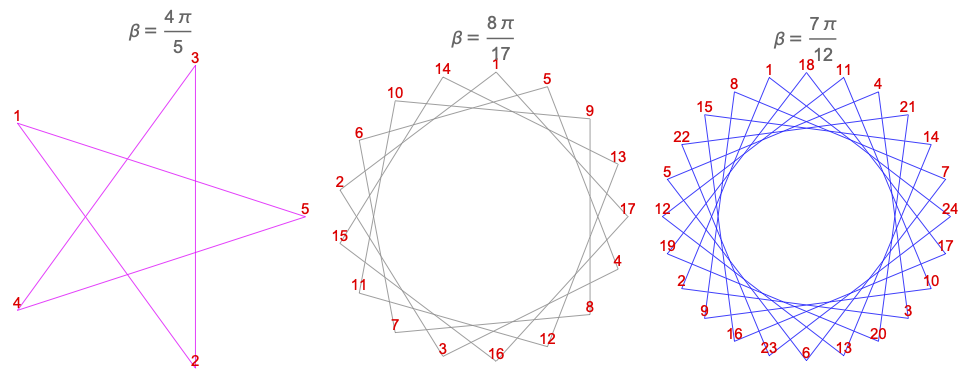
\includegraphics[width=0.62\columnwidth]{RegularPolygons.png}
    \caption{Examples of the regular star polygons $\{q/p\}$ that form the discrete target space of the momentum loop. The
    turbulent state, the Euler ensemble, is a statistical average over random walks on all such polygons (from
    Ref.~\cite{ReviewPaperAM}).}
    \label{fig:polygons}
\end{figure}

\paragraph*{Two ensembles.}
The continuum limit depends on the parity of $N$. In the odd-$N$ ensemble both $q$ and $r$ must be odd, whereas in the
even-$N$ ensemble at least one of them is even. The two limits are distinct superselection sectors, $\eta=N\bmod 2$, with a
different prime-$2$ Euler factor in the corresponding Mellin sums~\cite{migdal2026Riemann}. Only the odd ensemble is
marginally Lyapunov-stable in the statistical limit: it has infinitely many decaying modes and infinitely many zero modes.
The even ensemble is unstable~\cite{migdal2026EulerStability}. The odd ensemble is therefore the only marginally stable
turbulent attractor, and it is the one compared with experiment below.

\paragraph*{Universal energy spectrum.}
The Euler ensemble gives the decaying energy spectrum in the self-similar form~\cite{migdal2024quantum, migdal2026Riemann}
\begin{equation}
    E(k,t)=\frac{1}{L(t)}H\left(kL(t)\right),\qquad L(t)=\sqrt{\tilde\nu(t+t_0)},\qquad
    H(\kappa)=\int_{\epsilon-\I\infty}^{\epsilon+\I\infty}\frac{dp}{2\pi\I}\,M_\eta(p)\,\kappa^{p},
    \label{eq:Hkappa}
\end{equation}
with the parity-dependent Mellin amplitude
\begin{equation}
    M_\eta(p)=\frac{f(p)\,\Gamma(-p)\,\zeta\!\left(p+\frac{15}{2}\right)}
    {(2p+7)(2p+17)\,\zeta\!\left(p+\frac{17}{2}\right)\left(1-\eta\,2^{-(p+17/2)}\right)},\qquad \eta=N\bmod 2 ,
    \label{eq:Mtheor}
\end{equation}
where $f(p)$ is an entire function generated by the continuum limit of the Euler-ensemble path integral. It is independent
of the space dimension $d>1$~\cite{ReviewPaperAM}. The strip of the Mellin integral is $-7/2<\epsilon<0$. Besides the real
poles, $M_\eta$ has the Riemann wall $P_n=-8\pm\I\gamma_n$, $\zeta(\tfrac12+\I\gamma_n)=0$, paired with the zeros
$Z_n=-7\pm\I\gamma_n$. In the odd ensemble it also has the dyadic wall
$D_m=-\tfrac{17}{2}+2\pi\I m/\log 2$, $m\neq0$. When the Mellin integral~\eqref{eq:Hkappa} is evaluated by Lefschetz
thimbles, these walls generate the Stokes staircase of the energy spectrum: as $\log\kappa$ grows, the thimble traps the wall
poles one by one, each adding an exponentially small log-periodic correction $\kappa^{-8}\cos(\gamma_n\log\kappa+\phi_n)$ or
$\kappa^{-17/2}\cos(2\pi m\log\kappa/\log 2+\phi_m)$~\cite{migdal2026Riemann}.

\paragraph*{This paper.}
Experiments do not measure $E(k,t)$ at fixed $t$ over many decades; they measure the second-order structure function
$\VEV{(\Delta\vect v)^2}(r)$ and its local slope. Here we compute the effective index of the Euler-ensemble structure function
by the same thimble method used for the spectrum~\cite{migdal2026Riemann}. We work out its Stokes structure and add the
finite-size correction of a tunnel of finite width. We then compare the result with the Max Planck wind-tunnel
data~\cite{GregXi2} extrapolated to infinite Reynolds number.

\section{The method}\label{sec:method}

\subsection{Mellin--Barnes representation of the structure function}

Multiplying~\eqref{eq:Hkappa} by the three-dimensional kernel $\sin(k r)/(k r)$ and integrating over $k$ gives, with the
scaling variable $\rho=r/L(t)$ and $p=-1-q$,
\begin{align}
    G(\rho)&\equiv\int_0^\infty d\kappa\,H(\kappa)\frac{\sin\kappa\rho}{\kappa\rho}
    =\int_{c-\I\infty}^{c+\I\infty}\frac{dq}{2\pi\I}\,\rho^{q}\,Z_\eta(q),\qquad -1<c<0,\label{eq:Grho}\\
    Z_\eta(q)&=-\Gamma(-1-q)\cos\frac{\pi q}{2}\,M_\eta(-1-q)\nonumber\\
    &=-\frac{\pi}{2}\,\frac{\csc(\pi q/2)\,f(-1-q)\,\zeta\!\left(\frac{13}{2}-q\right)}
    {(1+q)(2q-15)(2q-5)\,\zeta\!\left(\frac{15}{2}-q\right)\left(1-\eta\,2^{q-15/2}\right)} ,
    \label{eq:Zq}
\end{align}
where $G(\rho)$ is the scaling function of the velocity correlation $\VEV{\vect v(0)\cdot\vect v(\vect r)}$.
The structure function $D(\rho)=2\left(G(0)-G(\rho)\right)$ is the same
integral with the contour shifted across the pole at $q=0$:
\begin{equation}
    D(\rho)=\int_{c'-\I\infty}^{c'+\I\infty}\frac{dq}{2\pi\I}\,\rho^{q}\,\left(-2Z_\eta(q)\right),\qquad 0<c'<2,
    \qquad \alpha(\rho)=\rho\,\partial_\rho\log D(\rho).
    \label{eq:Drho}
\end{equation}
The Gamma function $\Gamma(-p)$ of the spectrum is cancelled by the Fourier kernel $\Gamma(p)\sin(\pi p/2)$, leaving
$\csc(\pi q/2)$. Up to normalization, \eqref{eq:Zq} is the kernel $V(p)$ of Refs.~\cite{migdal2024quantum,ReviewPaperAM} for
$d=3$, with the odd-ensemble factor. Its poles in $q$ are:
\begin{itemize}
\item the real poles $q=-1$, $q=2n$ ($n\in\mathbb Z$), $5/2$, $11/2$, $15/2$ (a double pole in the odd ensemble) and $15/2+2n$
($n\ge1$);
\item the Riemann wall $7\pm\I\gamma_n$, with zeros at $6\pm\I\gamma_n$;
\item the dyadic wall $15/2\pm2\pi\I m/\log2$.
\end{itemize}
All complex singularities lie to the \emph{right}, at small $\rho$.

The entire function $f(p)$ is an integral over the polygon parameter $\Delta$,
\begin{equation}
    f(p)=20\int_{\Delta_1}^{\Delta_2}d\Delta\,(1-\Delta)\,C^{p-1}\left(AC-Bp\right),
    \label{eq:fp}
\end{equation}
with $A(\Delta),B(\Delta),C(\Delta)$ given in Ref.~\cite{migdal2024quantum}. We evaluate it on a fixed Gauss--Legendre grid in $\Delta$, which makes $f(p)$, $f'(p)$ and
$f''(p)$ exact and cheap for every complex $p$. Since $C(\Delta)\in[C_{\min},C_{\max}]=[e^{-2.915},e^{-2.763}]$, the factor
$f(-1-q)\sim C^{-2-q}$ fixes the convergence of the residue expansions:
\begin{itemize}
\item For $\rho>C_{\max}$ the contour closes to the left. $D(\rho)$ is then the convergent series
$D=2G(0)-2\left(a_1\rho^{-1}+\sum_{n\ge1}b_n\rho^{-2n}\right)$ in \emph{real} powers, and $\alpha(\rho)$ has no oscillatory component at all.
\item For $\rho<C_{\min}$ it closes to the right. $D=\sum_j c_j\rho^{q_j}$ over the right poles, and the only log-periodic terms
are $\rho^{7\pm\I\gamma_n}$ and $\rho^{15/2\pm2\pi\I m/\log2}$.
\end{itemize}
In the crossover $C_{\min}\lesssim\rho\lesssim C_{\max}$ neither series converges, and the integral must be computed directly.

\subsection{Lefschetz thimbles and Gauss--Hermite quadrature}

Write $-2Z_\eta(q)\rho^q=e^{W(q)}$, $W(q)=S(q)+q\log\rho$. For every $\rho$ there is one real saddle $q_0\in(0,2)$,
$W'(q_0)=0$, since $S''>0$ on the strip. As in Ref.~\cite{migdal2026Riemann}, the thimble through $q_0$ is parametrized so
that the weight decays as $e^{-t^2}$:
\begin{equation}
    W\left(q(t)\right)=W(q_0)-t^2,\qquad \frac{dq}{dt}=-\frac{2t}{W'(q)},\qquad
    q(\epsilon)=q_0+\epsilon v_0,\quad v_0=\I\sqrt{\frac{2}{W''(q_0)}},
    \label{eq:thimbleODE}
\end{equation}
with the lower branch $q(-t)=\overline{q(t)}$. The Gauss--Hermite rule with nodes and weights $\{t_j,w_j\}$ then gives
\begin{equation}
    D_{\rm thimble}(\rho)=\frac{e^{W(q_0)}}{\pi}\sum_{t_j>0}w_j\,\mathrm{Im}\,g(t_j),\qquad
    g(t)=e^{W(q(t))-W(q_0)+t^2}\,q'(t).
    \label{eq:GH}
\end{equation}
On an exact thimble the exponential factor in $g$ equals one. Keeping it makes~\eqref{eq:GH} exact by Cauchy's theorem even
where the numerical path drifts from the thimble, and doubles as a drift diagnostic. The effective index uses the same
nodes, $\rho\,\partial_\rho D_{\rm thimble}=\pi^{-1}e^{W(q_0)}\sum_{t_j>0}w_j\,\mathrm{Im}\left[q(t_j)g(t_j)\right]$, so no
numerical differentiation is needed. The ODE~\eqref{eq:thimbleODE} is integrated with the exact $S'(q)$, including $f'/f$.

\subsection{Stokes phenomenon: trapped poles and zero parking}

Because the complex walls of~\eqref{eq:Zq} lie to the right, the Stokes phenomenon of the structure function is the mirror
image of that of the spectrum. A pole $q_n$ is trapped between the vertical contour and the upper thimble when the rightward
ray $\{\mathrm{Im}\,q=\mathrm{Im}\,q_n,\ \mathrm{Re}\,q>\mathrm{Re}\,q_n\}$ crosses the thimble an odd number of times. The
orientation gives a minus sign:
\begin{equation}
    D(\rho)=D_{\rm thimble}(\rho)-2\,\mathrm{Re}\sum_{n\in\text{trapped}}\Res_{q=q_n}\left[-2Z_\eta(q)\rho^{q}\right],
    \label{eq:Stokes}
\end{equation}
with the Riemann-wall and dyadic-wall residues
\begin{align}
    \Res_{q=7+\I\gamma_n}&=\frac{\pi\,\rho^{q}\csc(\pi q/2)\,f(-1-q)\,\zeta\!\left(\frac{13}{2}-q\right)}
    {(1+q)(2q-15)(2q-5)\left(1-2^{q-15/2}\right)\left(-\zeta'\!\left(\frac{15}{2}-q\right)\right)},\\
    \Res_{q=15/2+2\pi\I m/\log2}&=\frac{\pi\,\rho^{q}\csc(\pi q/2)\,f(-1-q)\,\zeta\!\left(\frac{13}{2}-q\right)}
    {(1+q)(2q-15)(2q-5)\,\zeta\!\left(\frac{15}{2}-q\right)\,(-\log 2)} ,
\end{align}
checked against contour integrals around the poles to $10^{-12}$. The thimbles fall into three regimes (Fig.~\ref{fig:thimbles}):
\begin{enumerate}
\item For $\log\rho>-2.8$ the thimble bends to the left, where only real poles exist, and nothing is trapped. Near
$\log\rho\approx-2.87$ it rises almost vertically and reaches the walls only at heights $\mathrm{Im}\,q>80$, where the
residues are negligible.
\item For $-3.8\le\log\rho\le-2.95$ the thimble \emph{parks} on a zero $6+\I\gamma_n$ of $Z_\eta$, before reaching the Riemann
wall. The contour then continues up $\mathrm{Re}\,q=6$, contributing a tail smaller than $3\times10^{-14}$ in relative terms. The
index $n$ of the parking zero jumps $1,2,3,5,6,7,8,14,\ldots$ as $\log\rho\to-2.87$: this is the zero-parking staircase of the
structure function (Fig.~\ref{fig:staircase}).
\item For $\log\rho<-3.85$ the thimble escapes to the right below the first zero and traps the whole Riemann and dyadic walls
above its crossing height. The first dyadic pole, at height $2\pi/\log2=9.06$, is trapped for $\log\rho<-4.2$.
\end{enumerate}

\begin{figure}[t]
    \centering
    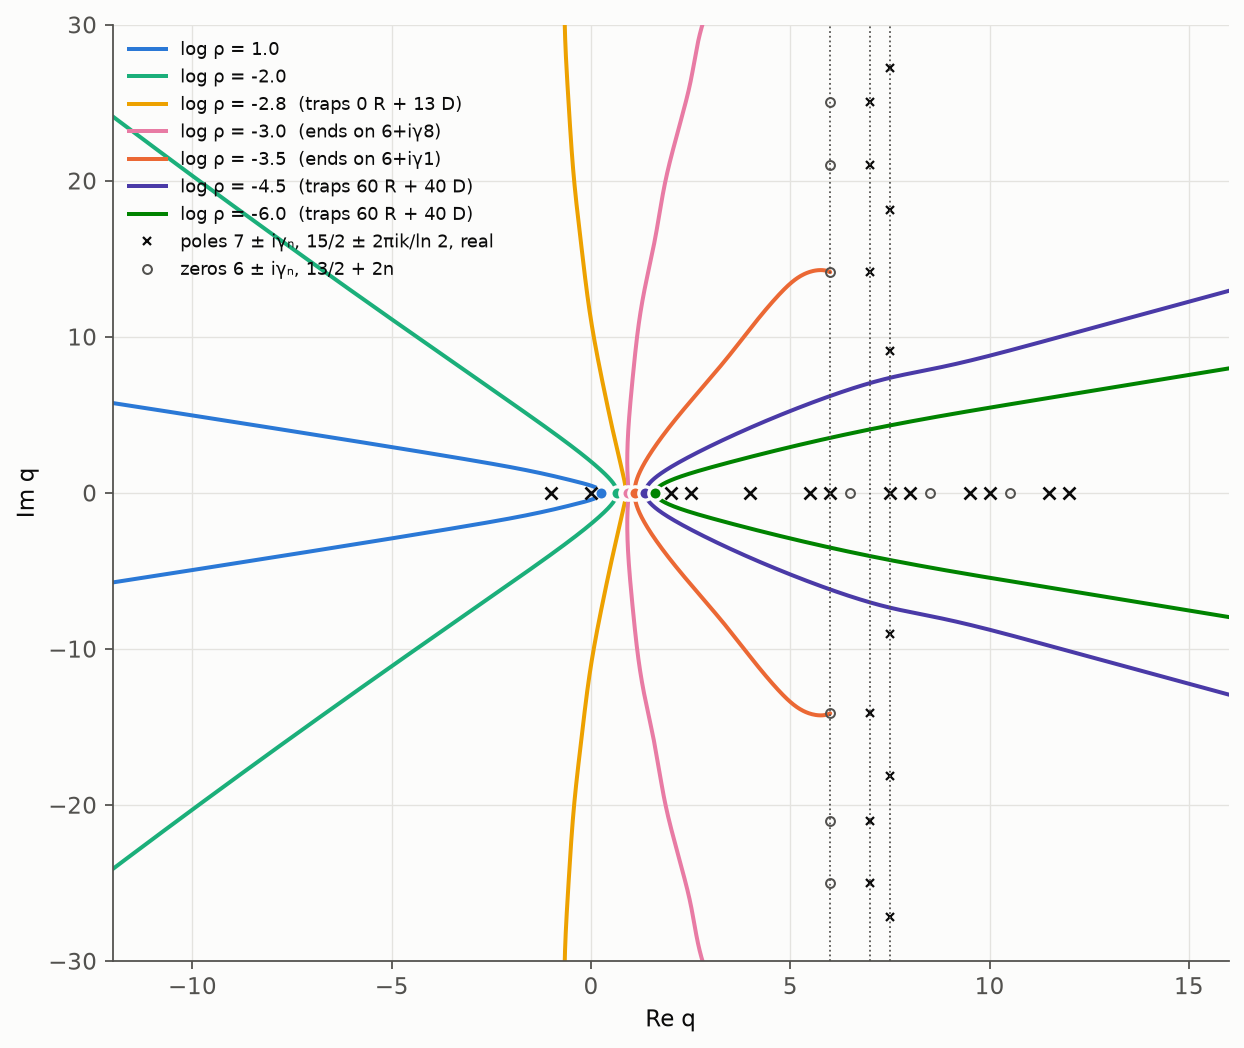
\includegraphics[width=0.78\columnwidth]{fig4_thimbles.png}
    \caption{Lefschetz thimbles of $\rho^{q}(-2Z_\eta(q))$ (odd ensemble) through the real saddles $q_0\in(0,2)$, for
    $\log\rho=1,-2,-2.8,-3,-3.5,-4.5,-6$. Crosses are poles: the Riemann wall $7\pm\I\gamma_n$, the dyadic wall
    $15/2\pm2\pi\I m/\log2$, and the real poles. Circles are the zeros $6\pm\I\gamma_n$ and $13/2+2n$. Dotted lines mark
    $\mathrm{Re}\,q=6,7,15/2$.}
    \label{fig:thimbles}
\end{figure}

\begin{figure}[t]
    \centering
    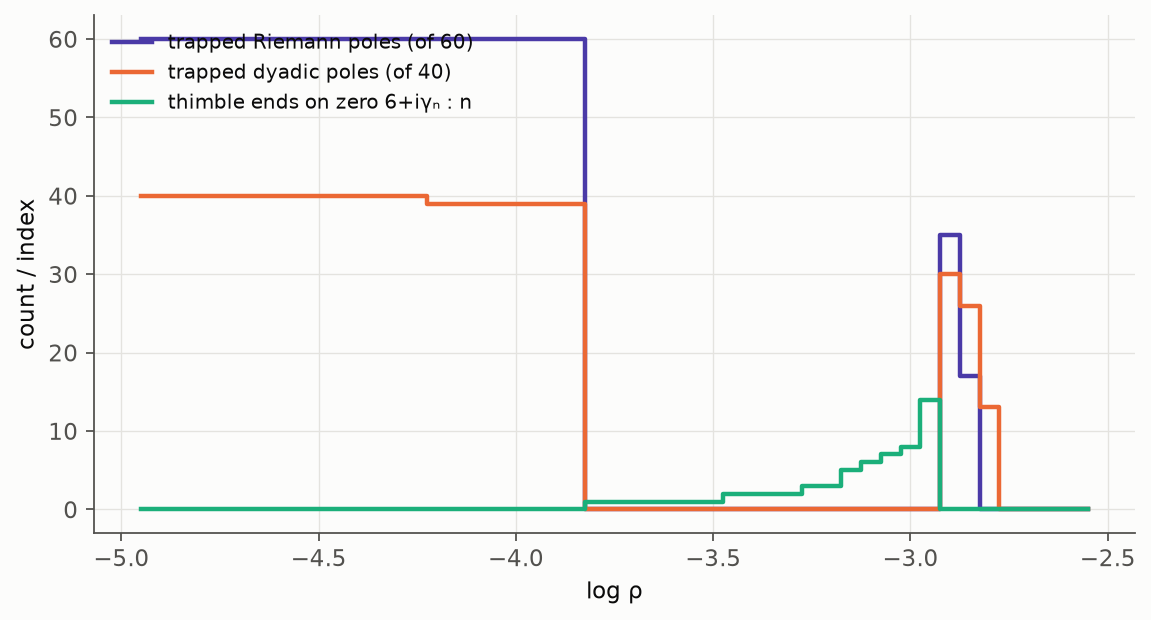
\includegraphics[width=0.78\columnwidth]{fig3_staircase.png}
    \caption{Stokes staircases of the structure function: the number of trapped Riemann poles (of $60$) and dyadic poles
    (of $40$), and the index $n$ of the zero $6+\I\gamma_n$ on which the thimble parks.}
    \label{fig:staircase}
\end{figure}

\subsection{Results for the infinite system}

With $80$ Gauss--Hermite nodes, the thimble plus Stokes terms~\eqref{eq:Stokes} reproduce the direct integration
of~\eqref{eq:Drho} along $\mathrm{Re}\,q=1$ over $-8\le\log\rho\le8$. The relative deviation is at most $5\times10^{-10}$ for
$D$, and the absolute deviation at most $4\times10^{-10}$ for $\alpha$ (Fig.~\ref{fig:Dalpha}). Apart from the tiny log-periodic corrections discussed below, the effective
index falls monotonically from the dissipative value $\alpha\to2$ at $\rho\to0$ to $\alpha\to0$ at $\rho\to\infty$, where
$\alpha=a_1/(G(0)\rho)+O(\rho^{-2})$. There is no inertial plateau: the whole crossover takes place within
$-5\lesssim\log\rho\lesssim0$.

\begin{figure}[t]
    \centering
    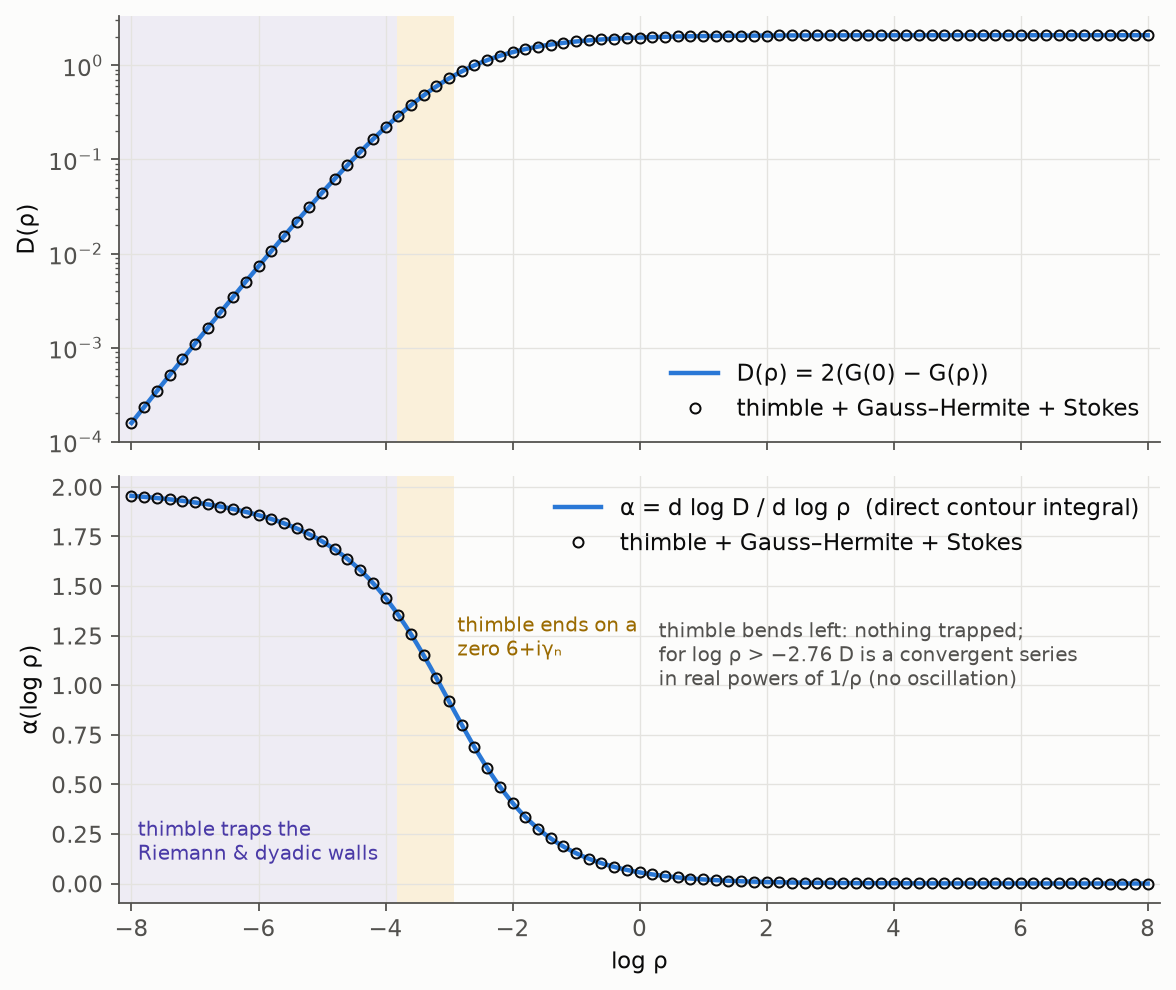
\includegraphics[width=0.8\columnwidth]{fig1_D_alpha.png}
    \caption{The structure function $D(\rho)$ and the effective index $\alpha(\rho)$ of the odd Euler ensemble (lines: direct
    contour integration; circles: thimbles with Gauss--Hermite quadrature and Stokes terms). The shaded bands mark the
    zero-parking (orange) and wall-trapping (violet) regimes.}
    \label{fig:Dalpha}
\end{figure}

\paragraph*{Oscillations of the structure function and of the spectrum.}
The log-periodic part of $\alpha$ is the sum of all wall residues. It is shown in Fig.~\ref{fig:osc}, together with the
log-periodic part of the spectral index $d\log H/d\log\kappa$ computed from the same walls of~\eqref{eq:Mtheor}. The
dyadic wall dominates both, with period $\log2$. Where every wall pole is trapped, the thimble's Stokes terms reproduce the
full wall sum to $10^{-12}$. The oscillations of $\alpha$ are at most $1.4\times10^{-6}$ (at $\log\rho=-3$, next to the edge of convergence) and fall as
$\rho^{5.5}$: they reach $2\times10^{-9}$ at $\log\rho=-4$ and $8\times10^{-11}$ at $\log\rho=-4.5$. At the same distance from
the convergence edge, the oscillations of the spectral index are eight to nine orders of magnitude larger (Fig.~\ref{fig:osc}).
The reason is the factor $\Gamma(-p)$ in $M_\eta(p)$. At the walls its power growth $|p|^{-\mathrm{Re}\,p-1/2}$ compensates
the exponential decay $e^{-\pi|\mathrm{Im}\,p|/2}$, for example $|\Gamma(\tfrac{17}{2}-2\pi\I/\log2)|=1.8\times10^{2}$. In
coordinate space this Gamma function is cancelled by the Fourier kernel, and only
$|\csc(\pi q/2)|=1.3\times10^{-6}$ remains at the first dyadic pole ($|\Gamma(8-\I\gamma_1)|=0.33$ against
$|\csc|=4.6\times10^{-10}$ at the first Riemann pole). The number theory of the Euler ensemble is thus clearly visible in the spectrum~\cite{migdal2026Riemann}
(Fig.~\ref{fig:spectrumStaircase}). The structure function has the same log-periodic oscillations, with the same periods:
$\log2$ in $\log\rho$ for the dyadic wall and $2\pi/\gamma_n$ for the Riemann wall. They appear only at small separations,
$\rho<C_{\min}$, the Fourier image of the large-$\kappa$ tail of the spectrum, and with amplitude at most $1.4\times10^{-6}$. At
large separations, $\rho>C_{\max}$, they are absent.

\begin{figure}[t]
    \centering
    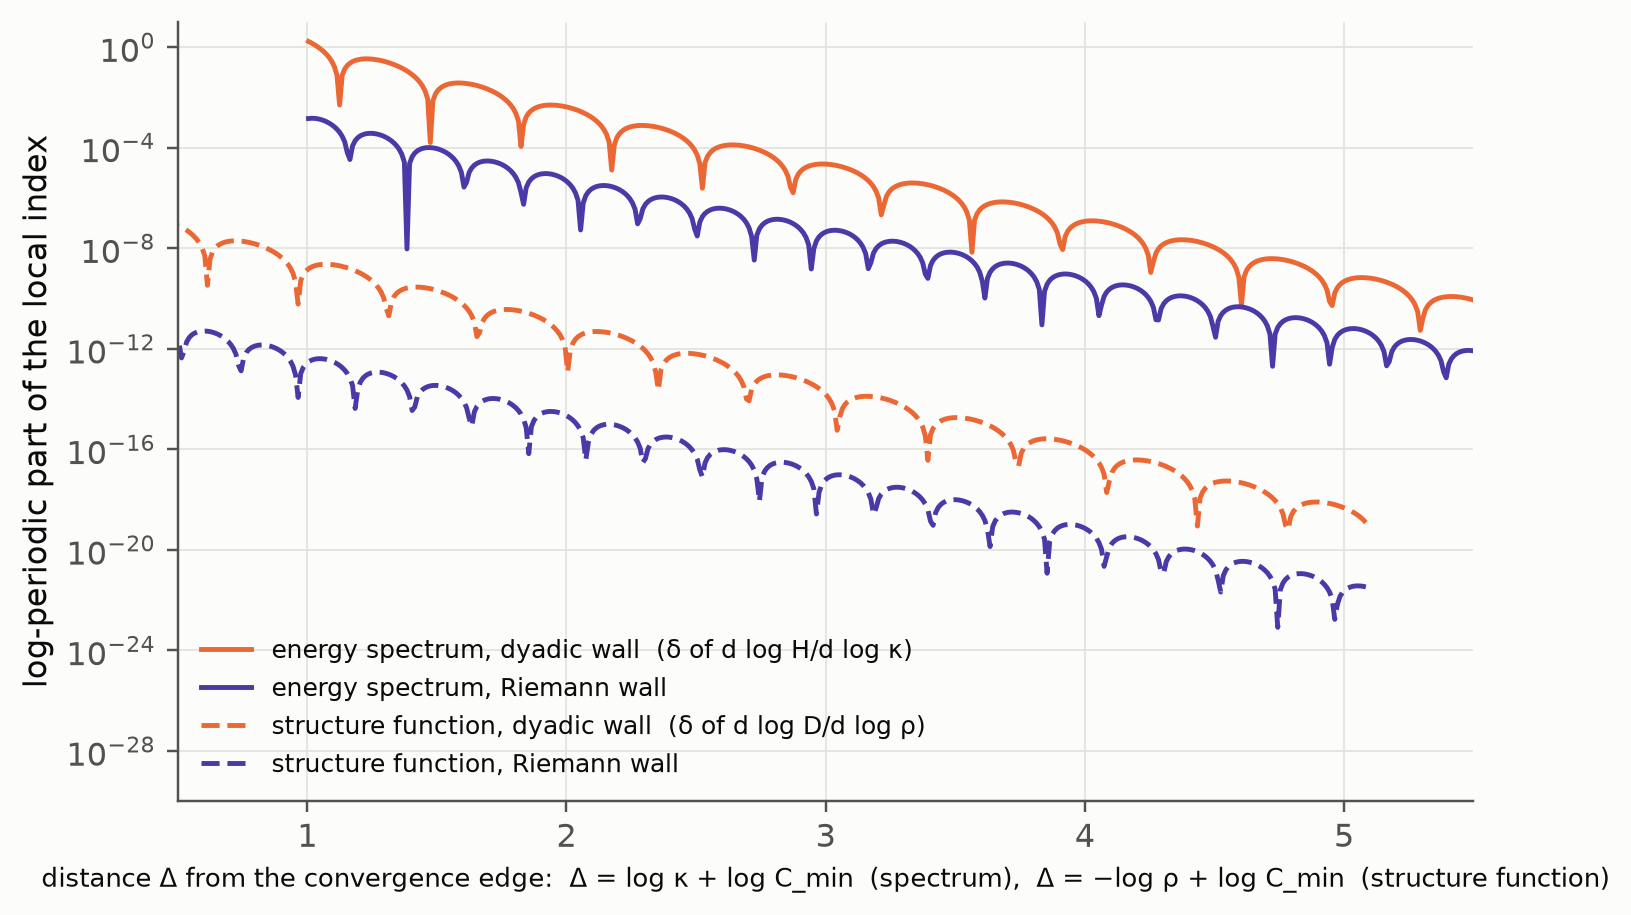
\includegraphics[width=0.8\columnwidth]{osc_compare.png}
    \caption{Log-periodic (wall-pole) part of the local index: energy spectrum, $\delta\left(d\log H/d\log\kappa\right)$ (solid),
    against structure function, $\delta\alpha$ (dashed), for the dyadic and Riemann walls of the odd ensemble. The horizontal
    axis is the distance from the edge of convergence of the corresponding residue series, $\log\kappa>-\log C_{\min}$ for the
    spectrum and $\log\rho<\log C_{\min}$ for the structure function.}
    \label{fig:osc}
\end{figure}

\begin{figure}[t]
    \centering
    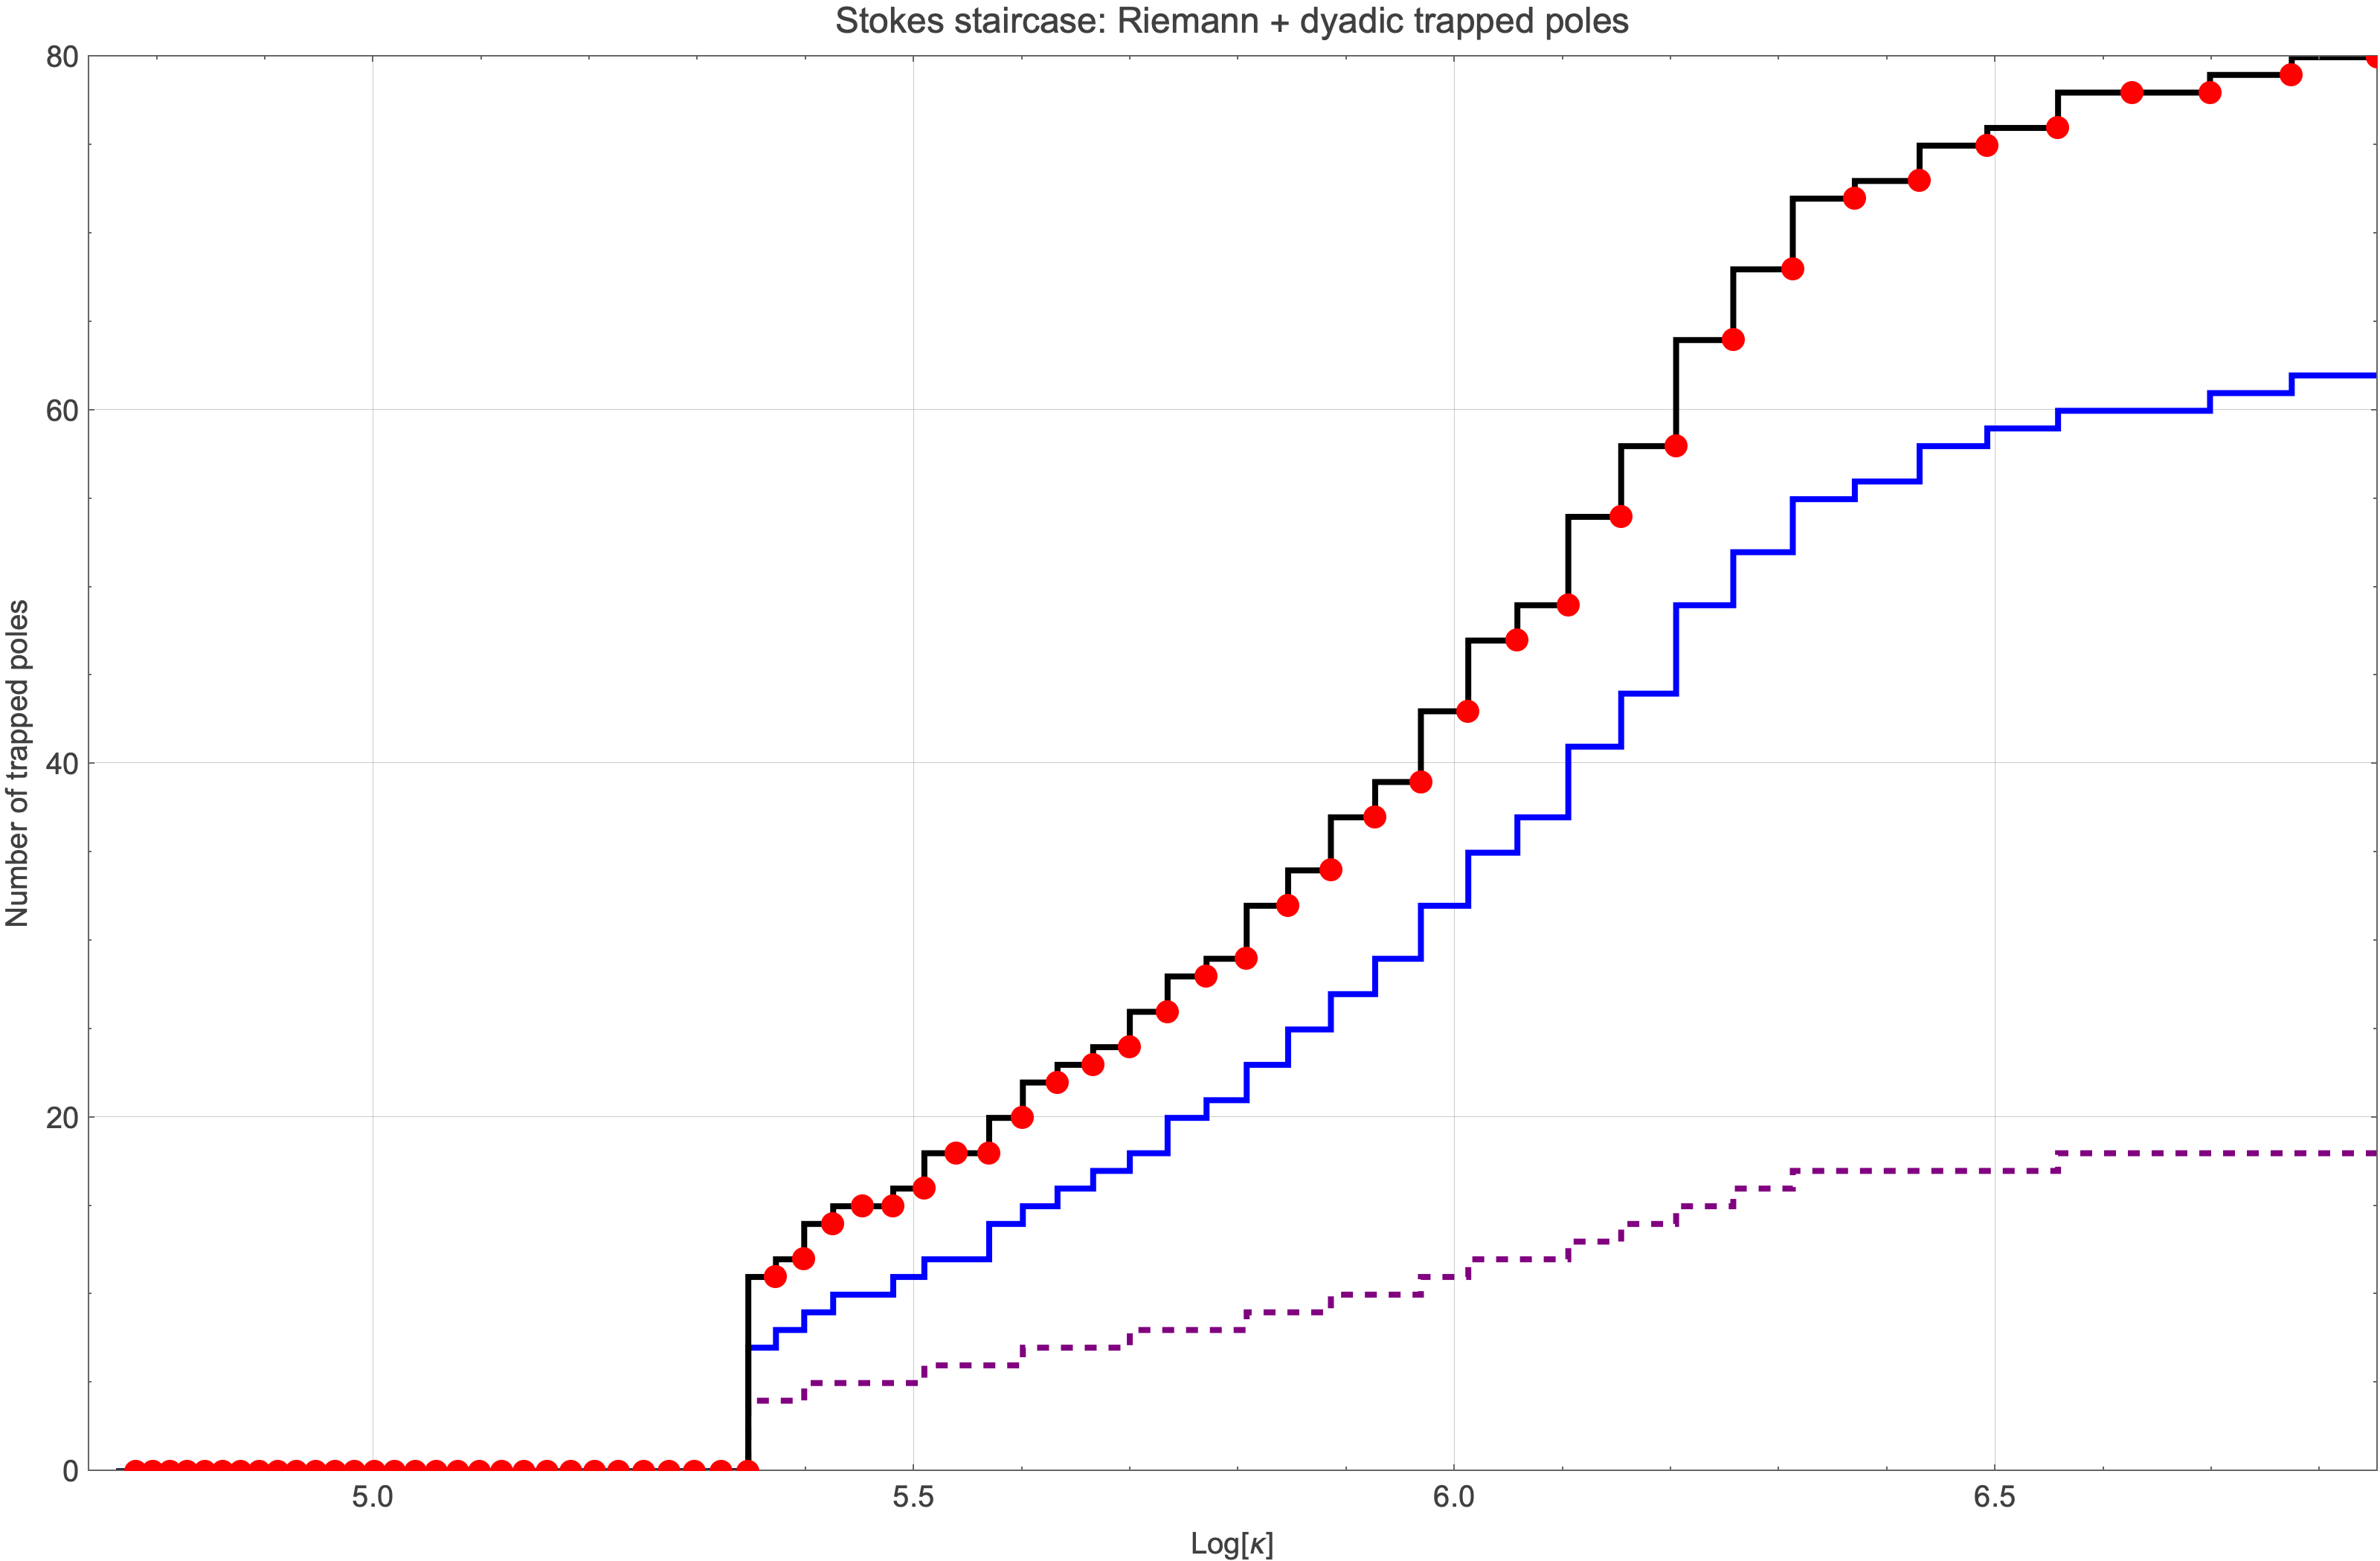
\includegraphics[width=0.66\columnwidth]{StokesOddStaircase.png}
    \caption{Stokes staircase of the energy spectrum in the odd Euler ensemble, from Ref.~\cite{migdal2026Riemann}: the
    total number of trapped poles (black, dots), Riemann-wall poles (blue) and dyadic-wall poles (dashed) as functions of
$\xi=\log\kappa$. Each trapped
    pole adds a log-periodic correction to $H(\kappa)$.}
    \label{fig:spectrumStaircase}
\end{figure}

\subsection{Finite-size correction}

The Euler ensemble describes homogeneous turbulence in infinite space. In a system of finite width $W$ the modes $k\lesssim\pi/W$
are absent or non-universal. In the scaling variables this is a cutoff $\kappa>\kappa_{\min}=\pi L(t)/W$, and the structure
function becomes
\begin{equation}
    D_W(\rho)=2\int_{\kappa_{\min}}^{\infty}d\kappa\left(1-\frac{\sin\kappa\rho}{\kappa\rho}\right)H(\kappa)
    =D(\rho)-2\int_0^{\kappa_{\min}}d\kappa\left(1-\frac{\sin\kappa\rho}{\kappa\rho}\right)H(\kappa).
    \label{eq:DW}
\end{equation}
The infinite-system $D(\rho)$ is the thimble result. The subtracted infrared part is computed from the small-$\kappa$
expansion of $H$. Closing the contour of~\eqref{eq:Hkappa} to the right, only the poles of $\Gamma(-p)$ contribute, and
\begin{equation}
    H(\kappa)=\sum_{n=0}^{\infty}\frac{(-\kappa)^n}{n!}A_n,\qquad
    A_n=\frac{f(n)\,\zeta\!\left(n+\frac{15}{2}\right)}{(2n+7)(2n+17)\,\zeta\!\left(n+\frac{17}{2}\right)\left(1-\eta\,2^{-(n+17/2)}\right)} .
    \label{eq:Hseries}
\end{equation}
Since $f(n)\sim C^{n}$, this is an entire function of $\kappa$. It reproduces the Mellin integral to $2\times10^{-14}$ for
$\kappa\le40$, and $\tfrac{\pi}{2}H(0)$ equals the large-$\rho$ coefficient $a_1$ of $G(\rho)$. The index
$\alpha_W=\rho\,\partial_\rho\log D_W$ uses
$\rho\,\partial_\rho\left(1-\sin x/x\right)=-\cos x+\sin x/x$. The lower endpoint of~\eqref{eq:DW} leaves a term
$\propto H(\kappa_{\min})\cos(\kappa_{\min}\rho)/(\kappa_{\min}\rho^2)$. As a result $\alpha_W$ oscillates about zero with period
$2\pi/\kappa_{\min}\approx2W/L$ in $\rho$, periodic rather than log-periodic, and first dips below zero near $\rho\approx W/L$
(Fig.~\ref{fig:box}). These are the only oscillations of the index at large separations. An earlier evaluation of the index
with the spectrum integrated over $0.1<\kappa<1000$~\cite{MB46} found exactly such oscillations at large $\rho$; they are the
finite-size oscillations of~\eqref{eq:DW} with $\kappa_{\min}=0.1$.

\begin{figure}[t]
    \centering
    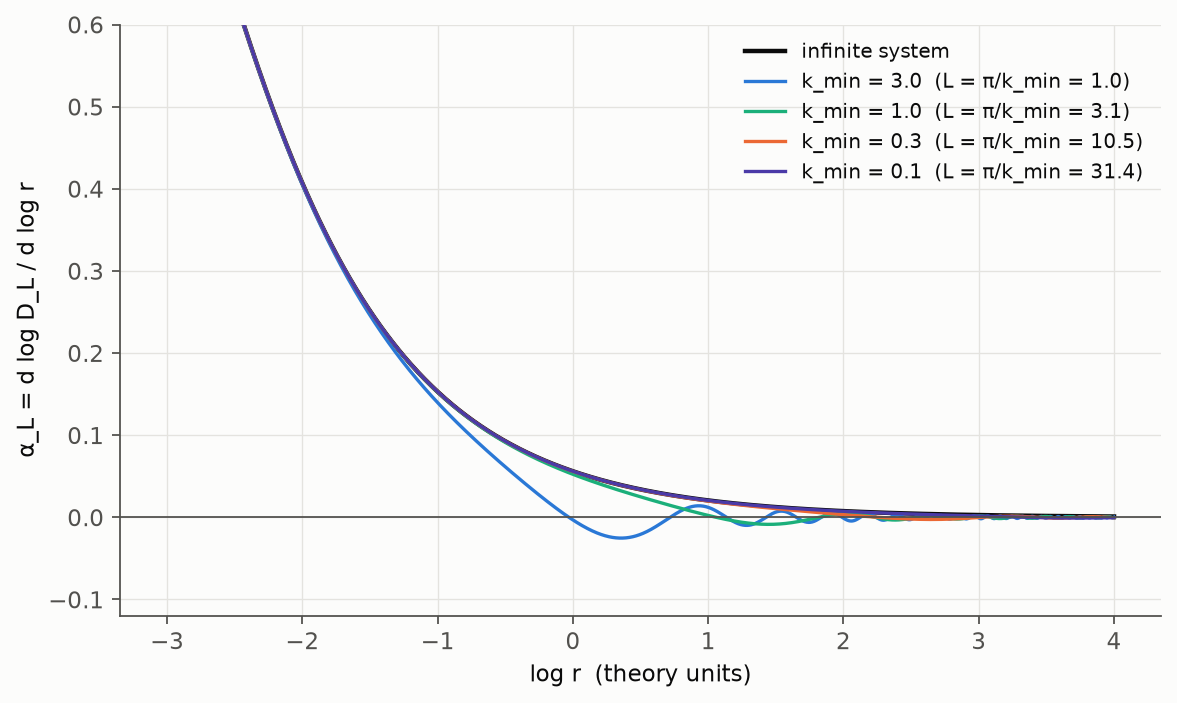
\includegraphics[width=0.8\columnwidth]{fig10_finite_box_theory.png}
    \caption{The effective index of the finite system, Eq.~\eqref{eq:DW}, for several infrared cutoffs $\kappa_{\min}=\pi L/W$,
    compared with the infinite system.}
    \label{fig:box}
\end{figure}

\section{Wind tunnel and DNS data}\label{sec:data}

\subsection{The Max Planck measurements}

We use the second-order structure functions $S_2(r)$ measured in decaying turbulence in the Max Planck Variable Density
Turbulence Tunnel by Küchler, Bewley and Bodenschatz~\cite{GregXi2}, for $11$ runs with $Re_\lambda=413$--$5779$. These are the
full data sets behind Ref.~\cite{GregXi2}, provided by the authors. The measured index is
$\alpha_{\exp}=d\log S_2/d\log r$, computed by centered differences. The unknown normalization of $S_2$ drops out of $\alpha$.

In grid turbulence the decay time is the distance from the grid, $t=z/\bar v_z$. The theory's variable is
$\rho=r/\ell_D$, with diffusion length $\ell_D=\sqrt{\tilde\nu(t+t_0)}$. The index depends only on $\rho$, so a single parameter per run, $s=\log(\ell_D/\eta)$, converts $r/\eta$ to $\rho$.
The files also give $u'$ and the Kolmogorov scale in physical units, assuming SI units for $S_2$ and $\epsilon$. The
viscosity inferred from $Re_\lambda$ and from the dissipation range agree to $1$--$20\%$, and $\eta$ ranges from $133\,\mu$m to
$8\,\mu$m. The integral scale $L=\int_0^{r_0}R\,dr$ of each run, with $R=1-S_2/2u'^2$, is $0.1$--$0.4$~m. The fitted diffusion
length is $\ell_D\approx(7$--$9)\,L$ in every run.

Each run's large-$r$ tail ($\alpha_{\exp}<0.355$, beyond the inertial plateau, which the theory does not contain) is fitted by
$\alpha(\rho)$ with rms deviation $0.014$--$0.045$. At the largest separations several runs show small oscillations of
$\alpha_{\exp}$, with dips to $-0.03\ldots-0.1$ (Fig.~\ref{fig:runs}). The infinite-system index cannot produce them: at these
separations, $\rho>C_{\max}$, it is positive and monotone, with no oscillations at all. The finite-width correction~\eqref{eq:DW}
reproduces them. With $\kappa_{\min}=\pi\ell_D/W$ fitted per run, the rms deviation drops by up to a factor of $2.5$. The
implied physical width is $W=2.25$--$2.6$~m for five of the seven runs with $Re_\lambda\le2398$, of the order of the largest
measured separations ($2.3$--$3.6$~m). A single $W=2.34$~m for these seven runs lowers their pooled rms deviation from $0.035$
to $0.023$. The runs with $Re_\lambda\ge3070$ show no dip and do not
constrain $\kappa_{\min}$. We conclude that the observed oscillations are finite-size effects. Their amplitude does not exceed the statistical scatter of
the data at the largest $r$, and they are not properties of decaying turbulence in infinite space.

\begin{figure}[t]
    \centering
    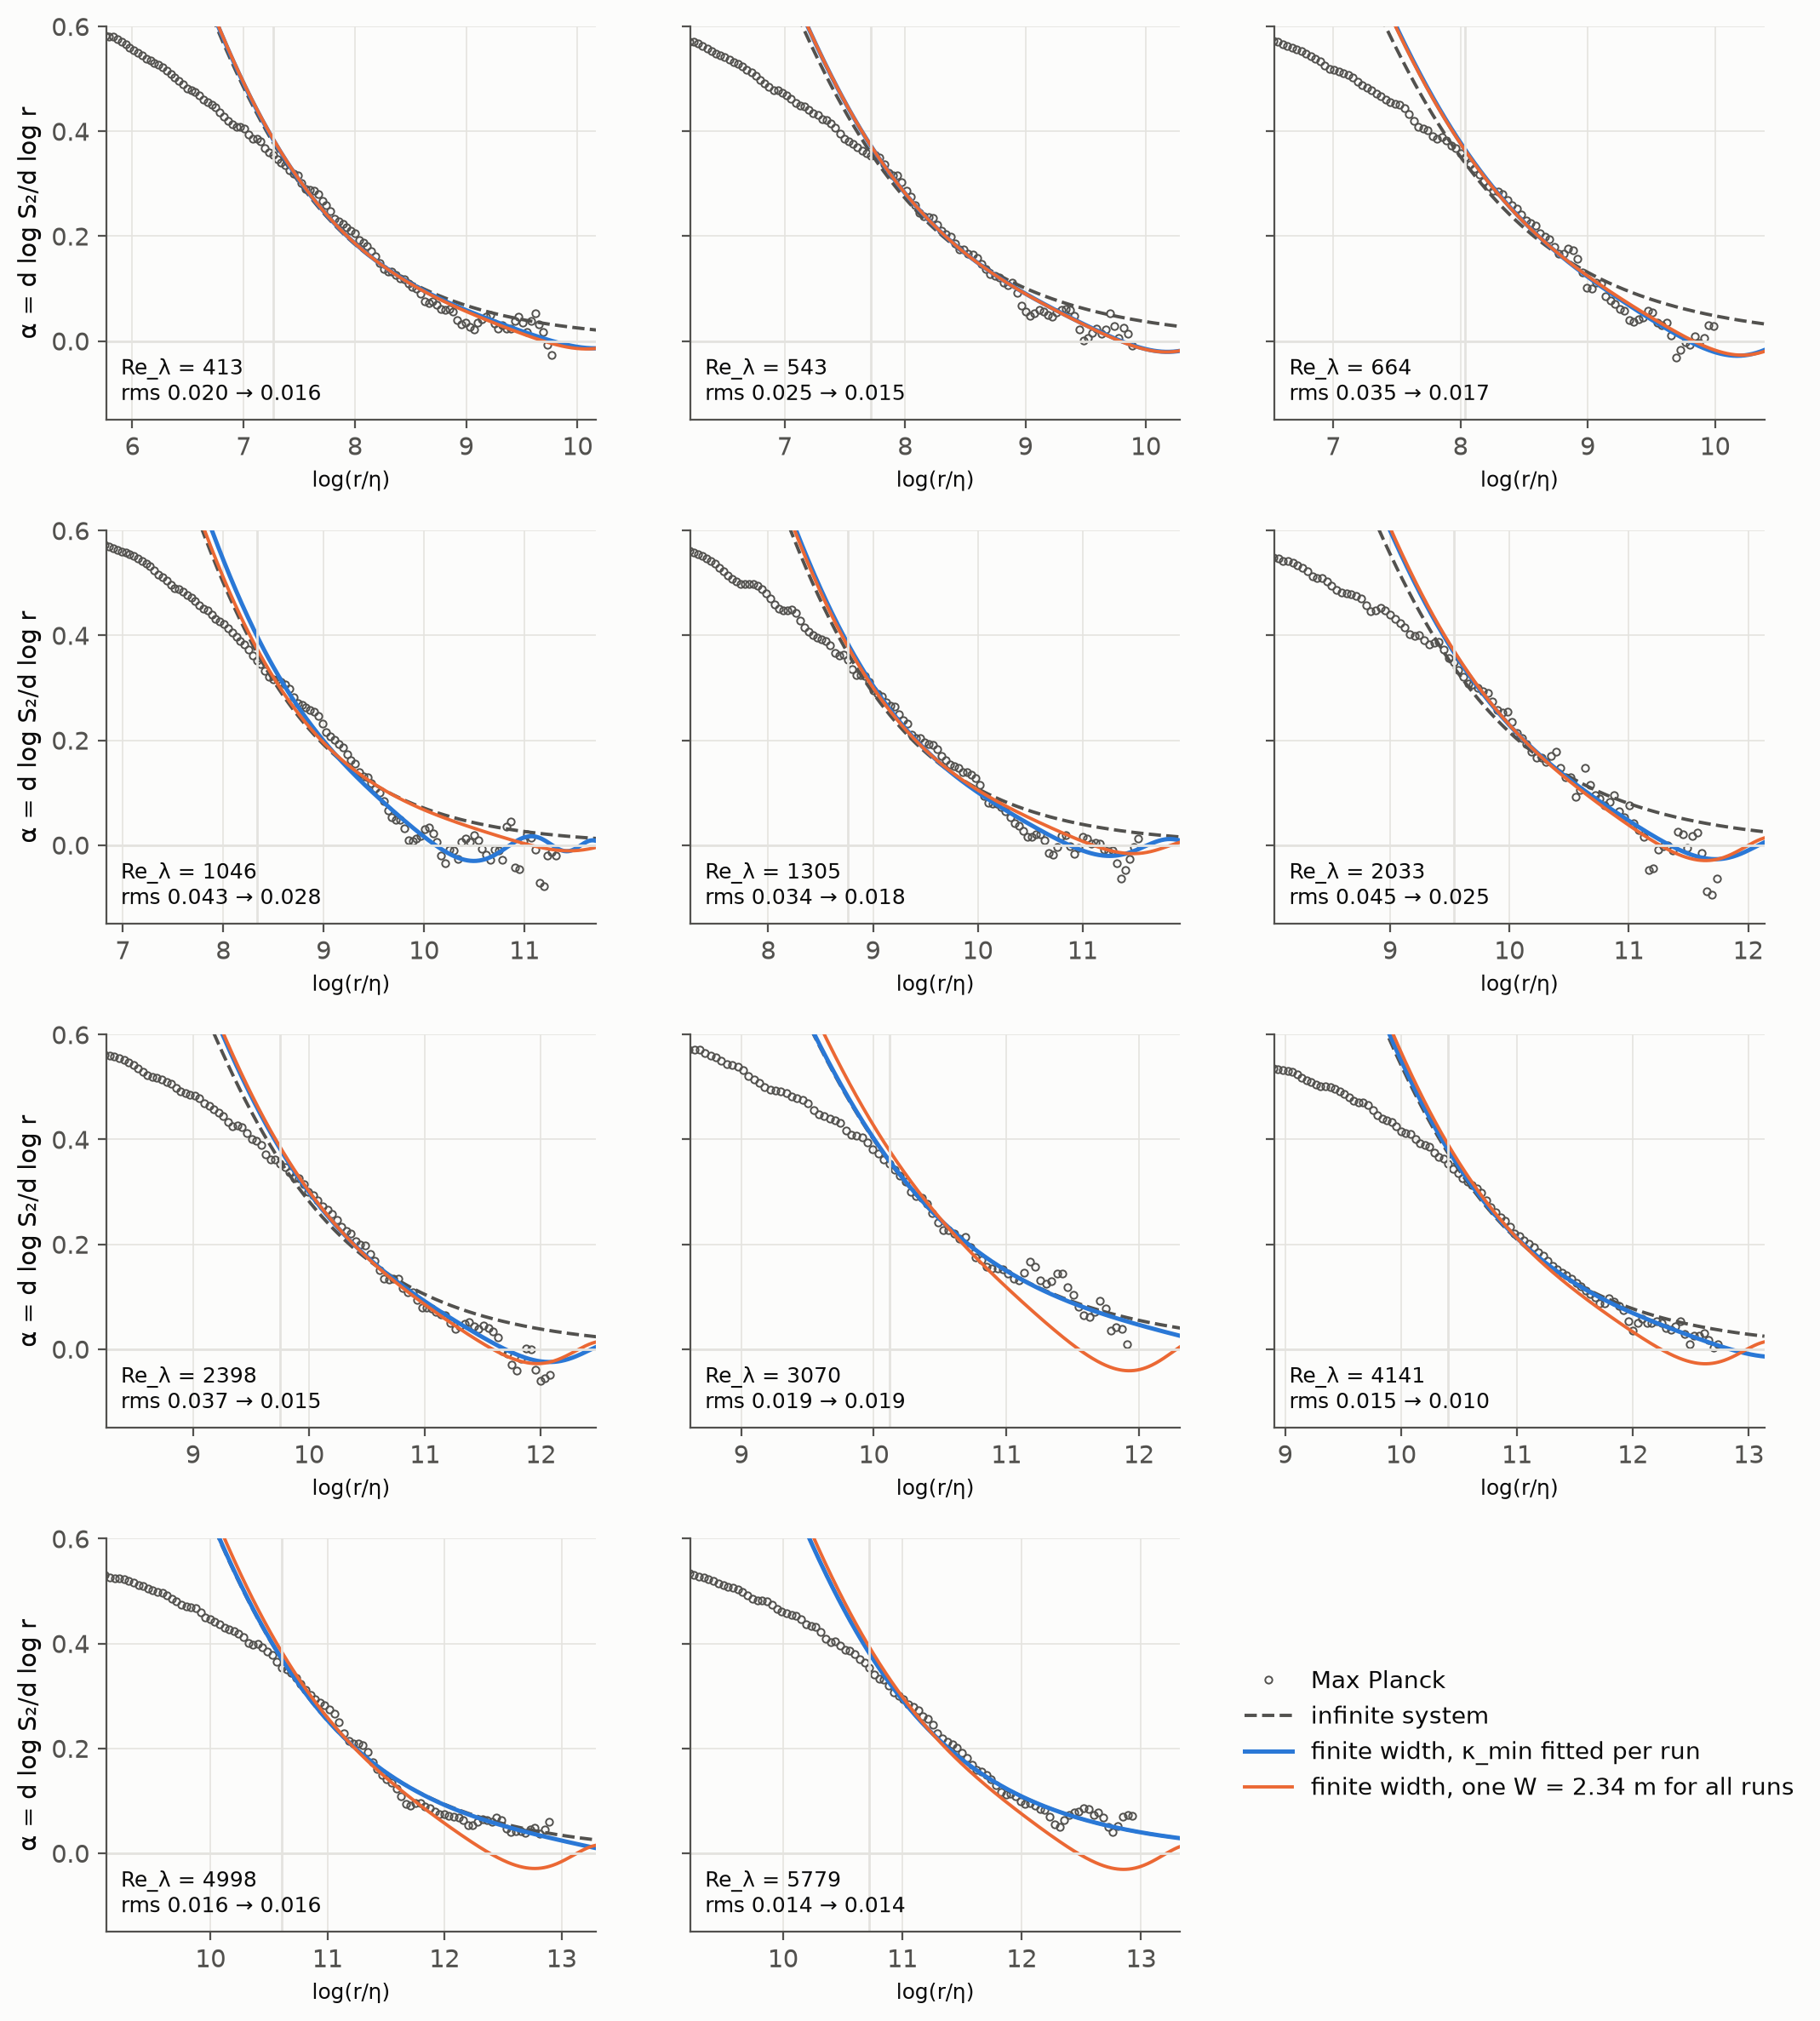
\includegraphics[width=\columnwidth]{fig9_finite_box_runs.png}
    \caption{Large-$r$ index of the Max Planck runs~\cite{GregXi2} (circles) against the infinite-system theory (dashed), the
    finite-width theory with $\kappa_{\min}$ fitted per run (blue), and one physical width $W=2.34$~m for all runs,
    $\kappa_{\min}=\pi\eta e^{s}/W$ (orange). The vertical line marks the start of the fitted tail. The labels give the rms
    deviation without and with the per-run finite-width correction.}
    \label{fig:runs}
\end{figure}

\subsection{Extrapolation to infinite Reynolds number}

The theory describes the limit $Re_\lambda\to\infty$. To compare with it we extrapolate the data, not the theory. Each run is
put on the data-defined scale $x=\log(r/L)$, and at fixed $x$ we fit
$\alpha_{\exp}(x,Re_\lambda)=\alpha_\infty(x)+c(x)/Re_\lambda$ over the mid- and high-Reynolds runs ($Re_\lambda\ge1046$). The
theory $\alpha(\rho)$ with $\log\rho=x-s$ is then fitted to the extrapolated tail $\alpha_\infty(x)<0.355$, with weights
$1/\sigma^2$ from the extrapolation. The result is shown in Fig.~\ref{fig:extrap}. A single parameter,
$s=\log(\ell_D/L)=1.956\pm0.021$ ($\ell_D/L=7.07\pm0.15$), gives $\chi^2/\mathrm{dof}=2.4$ and a weighted rms deviation of
$0.017$, with residuals within $\pm0.02$ over the whole tail. The finite-width term is no longer needed: fitted, it goes to
$\kappa_{\min}\to0.6$ without improving $\chi^2$. The negative dips of the individual runs do not survive the extrapolation,
which confirms that they are finite-size, finite-Reynolds effects.

Table~\ref{tab:extrap} shows the stability of the result under the choice of runs. The fit quality is stable. The scale ratio
$\ell_D/L$ drifts from $8.0$ to $6.2$ as the lower-Reynolds runs are dropped, more than its statistical error, so part of the
Reynolds dependence of the integral scale is not captured by the $1/Re_\lambda$ term. The even ensemble gives an index within
$0.0035$ of the odd one on this range and the same $\chi^2$ ($2.422$ against $2.423$), so the tail does not resolve the parity.
It is fully consistent with the odd ensemble, the only stable one.

\begin{table}[t]
    \centering
    \begin{tabular}{lccc}
    \toprule
    runs used & $s=\log(\ell_D/L)$ & $\chi^2/\mathrm{dof}$ & weighted rms of $\alpha$\\
    \midrule
    all $11$ ($Re_\lambda\ge413$) & $2.075\pm0.024$ & $2.8$ & $0.018$\\
    $Re_\lambda\ge1046$ (adopted) & $1.956\pm0.021$ & $2.4$ & $0.017$\\
    $Re_\lambda\ge1305$ & $1.943\pm0.020$ & $1.3$ & $0.015$\\
    $Re_\lambda\ge2033$ & $1.847\pm0.015$ & $1.9$ & $0.016$\\
    $Re_\lambda\ge2398$ & $1.823\pm0.017$ & $2.0$ & $0.012$\\
    \bottomrule
    \end{tabular}
    \caption{Fit of the odd-ensemble index to the Max Planck data extrapolated to $Re_\lambda\to\infty$ in $1/Re_\lambda$, for
    different sets of runs.}
    \label{tab:extrap}
\end{table}

\begin{figure}[t]
    \centering
    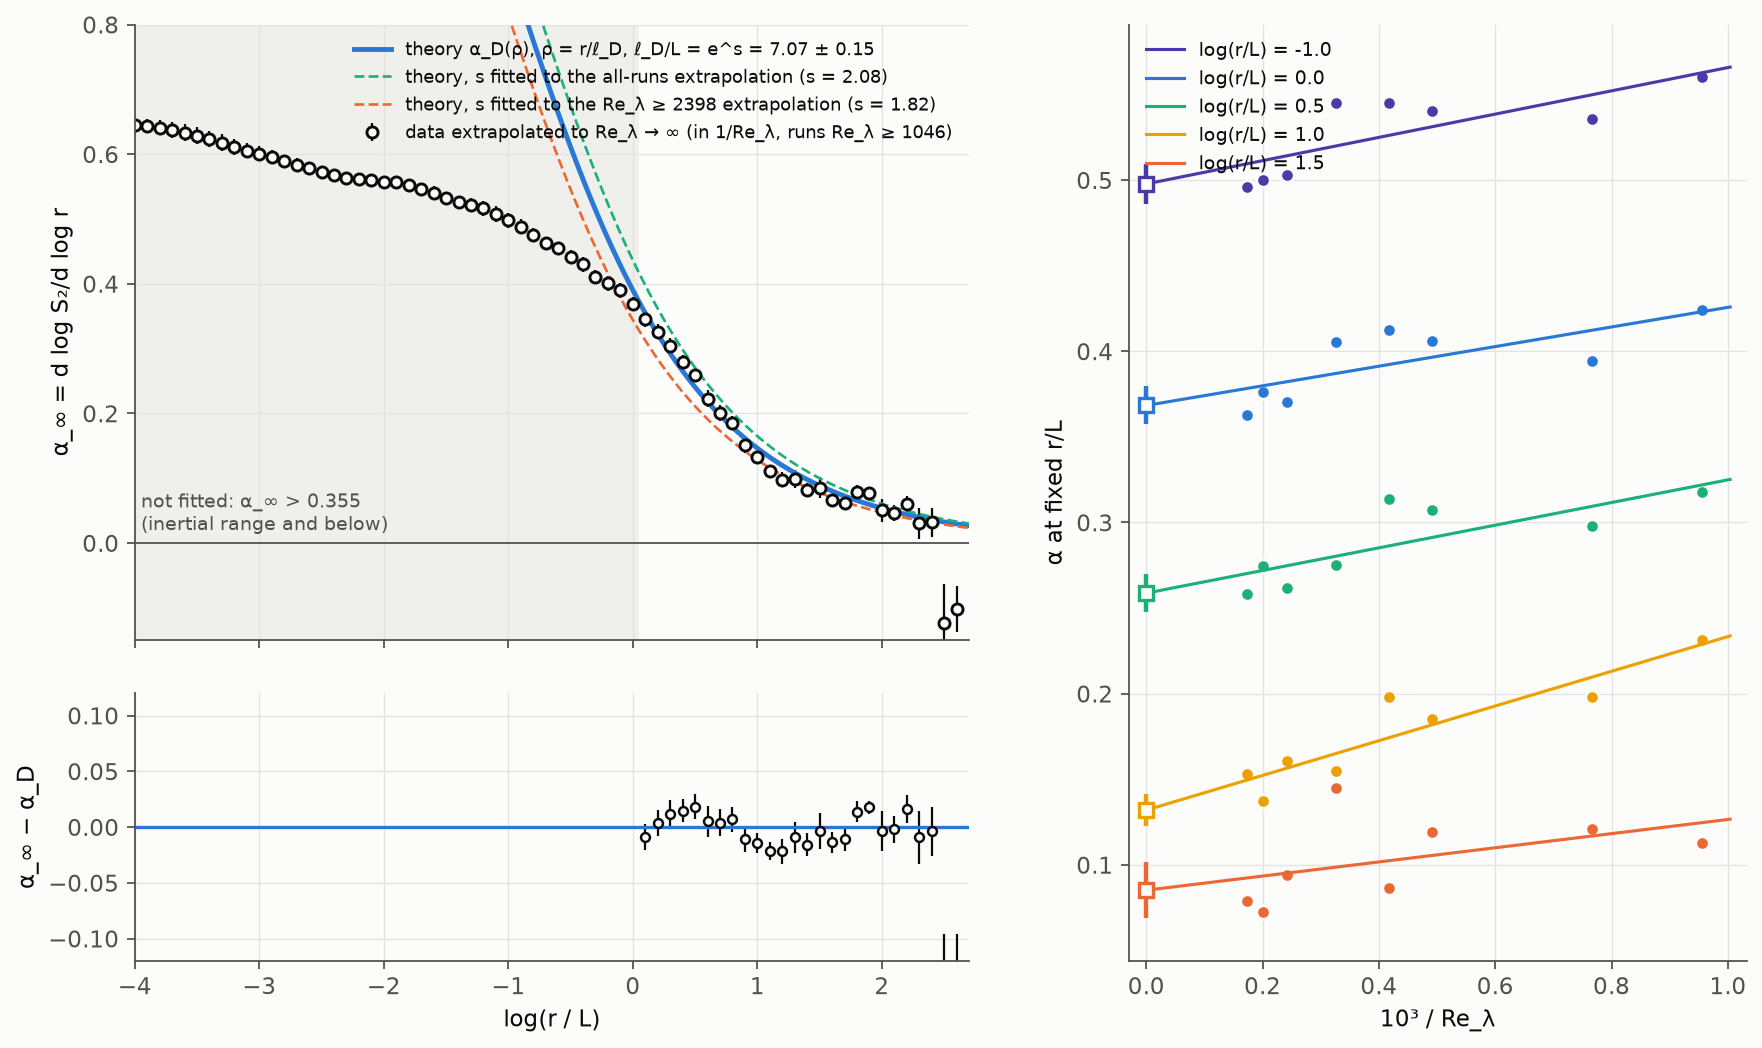
\includegraphics[width=\columnwidth]{fig13_invRe_extrapolation.png}
    \caption{Left: the Max Planck index extrapolated to $Re_\lambda\to\infty$ in $1/Re_\lambda$ (circles, runs
    $Re_\lambda\ge1046$) against the odd-ensemble theory with one scale parameter (blue). Dashed lines use the shifts fitted to
    the extrapolations with all runs and with $Re_\lambda\ge2398$ only. The fit uses the tail outside the shaded region; the
    residuals are shown below. Right: $\alpha_{\exp}$ against $1/Re_\lambda$ at fixed $r/L$; squares are the extrapolated
    values.}
    \label{fig:extrap}
\end{figure}

\subsection{Direct numerical simulation}

The same theoretical index has been compared with the $4096^3$ DNS of freely decaying turbulence by Rodhiya and
Sreenivasan~\cite{SreeniAkash2025}, where the time dependence is available directly and the scaling variable is
$r/L(t)$~\cite{ReviewPaperAM}. The parameter-free theory reproduces the whole nonlinear curve of the effective index
(Fig.~\ref{fig:dns}). The deviations at the largest $r/L$ come from the finite box and from early times, when $L(t)$ is still
small~\cite{ReviewPaperAM}. They are the numerical counterpart of the finite-width effect in the wind tunnel.

\begin{figure}[t]
    \centering
    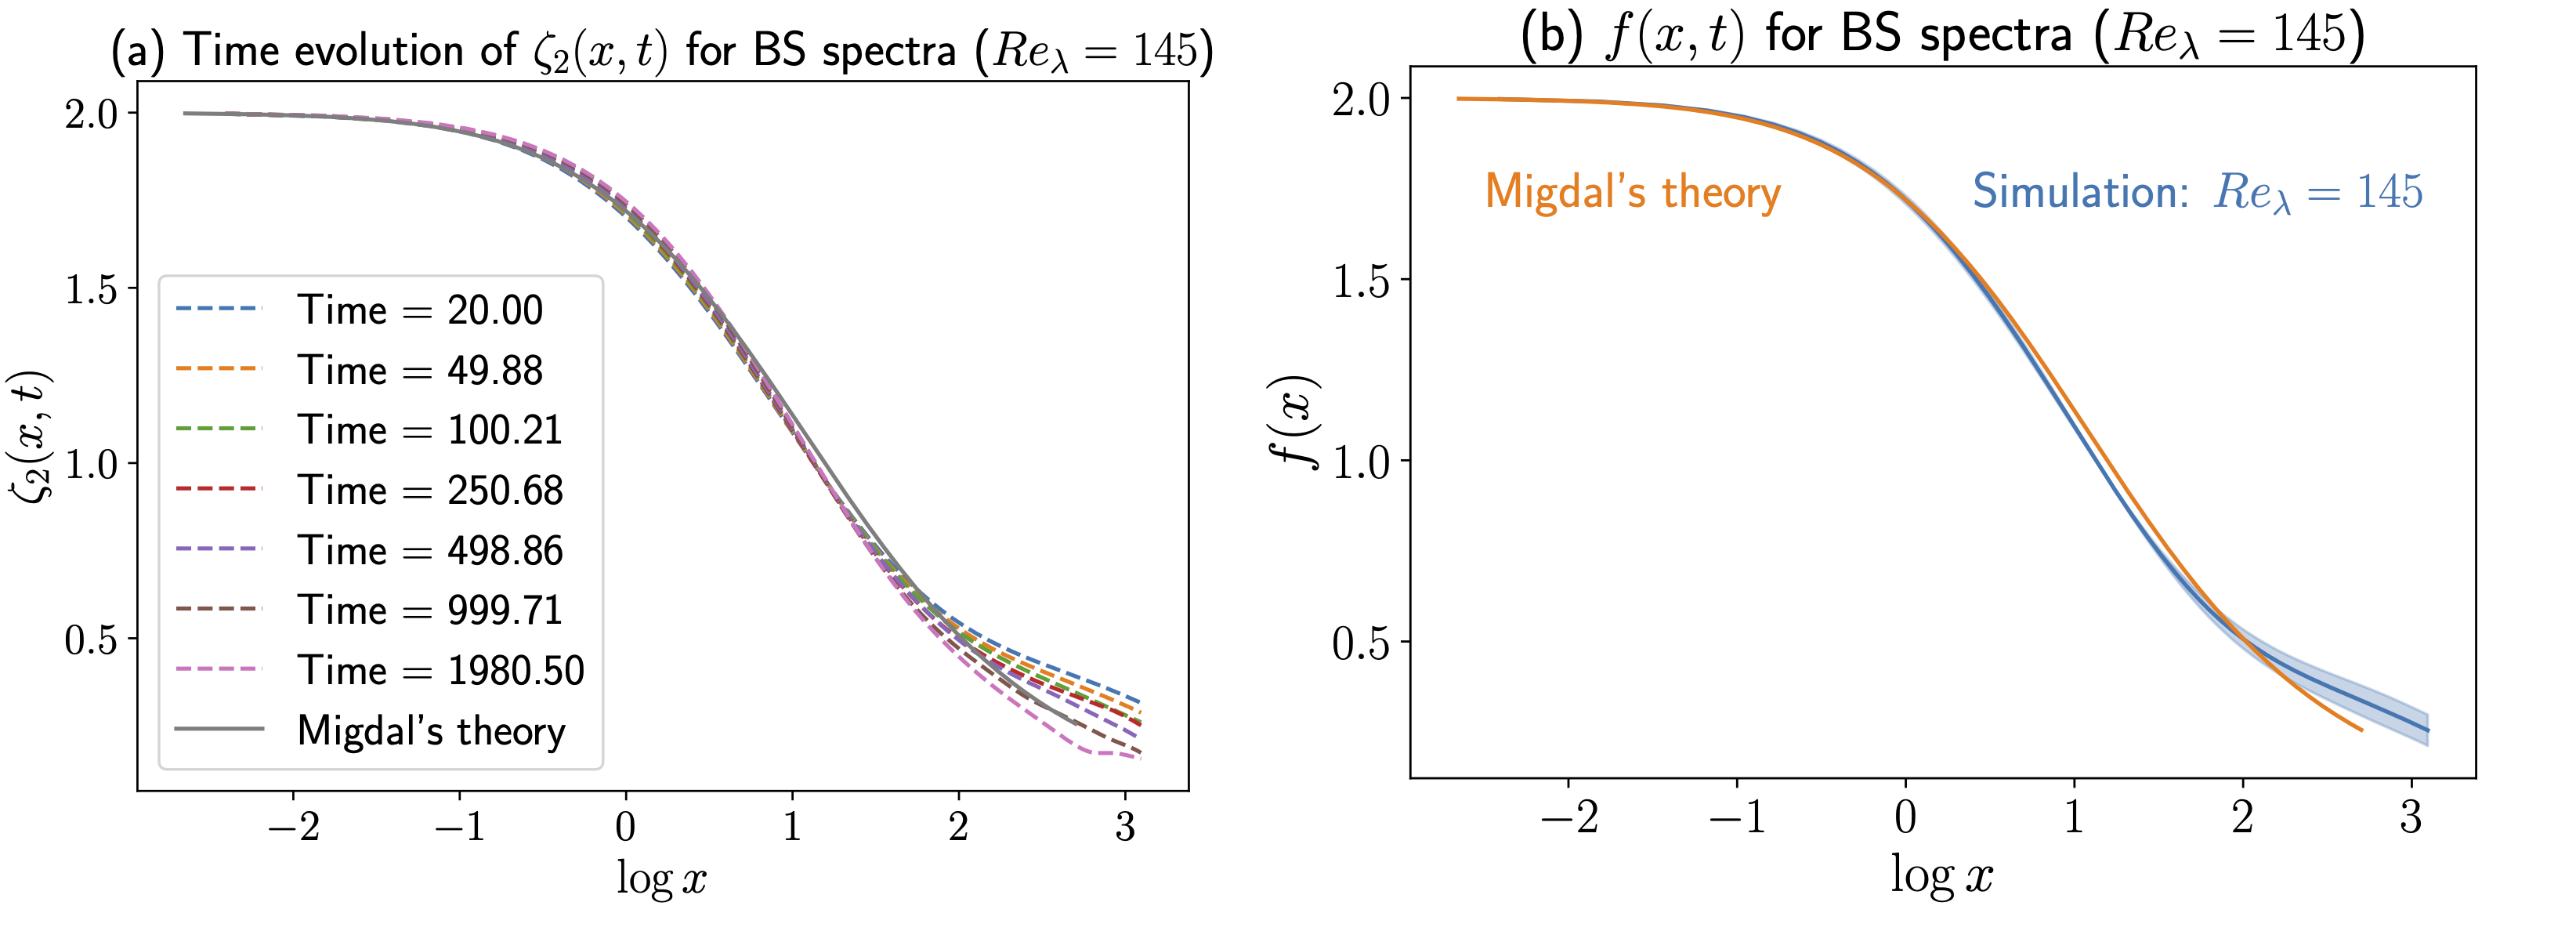
\includegraphics[width=0.72\columnwidth]{BSSpectra_clean.png}
    \caption{Effective index $\VEV{r\,\partial_r\log(\Delta v^2)}$ of the $4096^3$ DNS of decaying turbulence by Rodhiya and
    Sreenivasan~\cite{SreeniAkash2025} (Birkhoff--Saffman initial spectrum) against the Euler-ensemble prediction (from
    Ref.~\cite{ReviewPaperAM}).}
    \label{fig:dns}
\end{figure}

\subsection{Why only the tail of the index is compared}\label{sec:tail}

The comparison of Secs.~\ref{sec:data}\,A--B uses only the large-$r$ tail, $\alpha_{\exp}<0.355$, that is $r\gtrsim L$. At
smaller separations the measured index lies far below the theory (the shaded region of Fig.~\ref{fig:extrap}). At $r=L/e$ the
extrapolated index is $\alpha_\infty=0.50\pm0.01$ against the predicted $0.89$, and at $r=e^{-4}L$ it is $0.65\pm0.01$ against
$1.85$. The data have an inertial plateau, $\alpha_{\exp}\approx0.6$--$0.7$, which the theory does not contain: its index
decreases monotonically from $2$ to $0$ within $-5\lesssim\log\rho\lesssim0$.

The finite width of the tunnel cannot produce this difference. The correction~\eqref{eq:DW} removes only the wave numbers
$\kappa<\kappa_{\min}$. Even for the largest fitted $\kappa_{\min}\approx3.6$ it changes $\alpha$ by less than $10^{-3}$ for
$\log\rho\le-3$ and by $0.02$ at $\log\rho=-1$, while the observed differences are $0.4$--$1.2$. Nor is the difference a
finite-Reynolds correction that disappears as $1/Re_\lambda$ at fixed $r/L$. At fixed $r/L<1$ the measured index moves \emph{away}
from the theory as the Reynolds number grows: at $r=e^{-4}L$ it falls from $0.79$ at $Re_\lambda=1046$ to $0.66$ at
$Re_\lambda=5779$, because the plateau widens toward small $r/L$ as $L/\eta$ grows. The extrapolation in $1/Re_\lambda$ is
therefore meaningful only in the tail, where the Reynolds dependence at fixed $r/L$ is weak (Fig.~\ref{fig:extrap}, right).

The reason is the second length of the experimental flow. Küchler \emph{et al.} found that for
$10^2\eta<r<10^4\eta$ the index is a Reynolds-independent function of $r/\eta$~\cite{GregXi2}. In units of $L$ this range
extends over all $r<L$ at $Re_\lambda\approx10^3$, where $L\approx3\times10^3\eta$, and over $r\lesssim0.2L$ at
$Re_\lambda=5779$, where $L\approx4\times10^4\eta$. At fixed $r/L$ it therefore moves with the Reynolds number and recedes
only as $L/\eta\propto Re_\lambda^{3/2}$ grows; a $1/Re_\lambda$ extrapolation at fixed $r/L$ cannot remove it. The Euler
ensemble has a single length, the diffusion length $\ell_D=\sqrt{\tilde\nu(t+t_0)}$, and describes the asymptotic state of
the decay, $t\to\infty$, in which $\ell_D$ and the integral scale grow together as $\sqrt t$. The wind-tunnel flow is measured
at one station, $8.3$~m downstream of the active grid, after a finite decay time, with an integral scale that stays
approximately constant along the test section~\cite{GregXi2}. It has not reached the self-similar diffusive state, and its
small scales still carry the inertial range produced by the grid. The DNS of Sec.~\ref{sec:data}\,C, followed over very long
times~\cite{SreeniAkash2025}, has reached this state and reproduces the whole index curve. We therefore attribute the
mismatch at $r<L$ to the finite Reynolds number and the finite age of the wind-tunnel flow, which in decaying turbulence
are two sides of the same approach to the attractor, and not to the finite width. The tail $r\gtrsim L$ is the part of the
measured index that has already relaxed to the asymptotic state. This interpretation can be tested: at fixed Reynolds number,
measurements at increasing distance from the grid should show the agreement with the theory extending from the tail
toward smaller $r/L$, together with the growth $L\propto\sqrt t$.

\section{Conclusion}

The steepest-descent evaluation of the Mellin--Barnes integral, with Lefschetz thimbles, Gauss--Hermite quadrature and the
Stokes phenomenon, gives the Euler-ensemble structure function and its effective index with a relative accuracy better than
$10^{-9}$. The same
Riemann and dyadic walls that produce the Stokes staircase and the log-periodic oscillations of the energy
spectrum~\cite{migdal2026Riemann} are present in the structure function. There the Fourier kernel cancels the Gamma function
that makes them visible in the spectrum. The index therefore has log-periodic oscillations with the same periods, but only at
small separations, $\rho<C_{\min}$, and with amplitude below $1.5\times10^{-6}$. At large separations, where the structure
function is a convergent series in real inverse powers of $\rho$, they vanish identically.

The small-$\rho$ structure has a direct meaning in time. Since $\rho=r/\sqrt{\tilde\nu(t+t_0)}$, the limit $\rho\to0$ is
reached at small separations for fixed $t$ or, within the validity of the Navier--Stokes description, at fixed $r$ for
$t\to\infty$. For $\rho<C_{\min}$ the structure function is the convergent sum of its right residues,
\begin{equation}
    D(\rho)=\sum_j c_j\,\rho^{q_j}+\sum_{n}2\,\mathrm{Re}\left[R_n\,\rho^{7+\I\gamma_n}\right]
    +\sum_{m\ne0}2\,\mathrm{Re}\left[R'_m\,\rho^{15/2+2\pi\I m/\log2}\right],
    \label{eq:smallrho}
\end{equation}
where $q_j=2,\tfrac52,4,\tfrac{11}{2},6,\ldots$ are the real poles. At fixed $r$ the wall terms oscillate in $\log t$ with the
frequencies $\gamma_n/2$, set by the non-trivial zeros of $\zeta(s)$, and $\pi m/\log2$, set by the prime-$2$ Euler factor of the
odd ensemble. Their amplitude relative to the leading term decreases as $\rho^{5}\propto t^{-5/2}$. This infinite set of
incommensurate complex exponents makes $t=\infty$, equivalently $\rho=0$, an essentially singular point of the structure
function, exactly as $\kappa=\infty$ is for the energy spectrum~\cite{migdal2026Riemann}. Under $p=-1-q$ the exponents
$-8\pm\I\gamma_n$ and $-\tfrac{17}{2}\pm2\pi\I m/\log2$ of the spectrum map one to one onto $7\mp\I\gamma_n$ and
$\tfrac{15}{2}\mp2\pi\I m/\log2$. The infinite-time singularity of the velocity structure function is therefore dictated by the
same number theory as the spectral singularity. Only the order of the Stokes activations differs. In the spectrum the thimble
captures the Riemann-wall poles one by one, at times $t_n\propto\gamma_n^3/(\tilde\nu k^2)$ at fixed
$k$~\cite{migdal2026Riemann}. In the structure function, where the Fourier kernel cancels $\Gamma(-p)$, the thimble captures
the whole walls at once, for $\log\rho\lesssim-3.85$. In both representations the singular structure of decaying turbulence at
infinite time is encoded by the zeros of the Riemann zeta function: number theory decodes turbulent intermittency.

The small oscillations of the index observed at the largest separations in the Max Planck wind tunnel are reproduced by the
finite width of the tunnel. They disappear when the data are extrapolated to infinite Reynolds number, and they are of the
order of the statistical scatter or below it. They are not a property of decaying turbulence in infinite space. The extrapolated tail of
the measured index matches the odd Euler ensemble, the only stable turbulent attractor, with a single scale parameter. The
$4096^3$ DNS reproduces the whole index curve. At smaller separations the measured index shows an inertial plateau that the
theory does not contain. It is not a finite-size effect, and it is not a finite-Reynolds correction that vanishes as
$1/Re_\lambda$ at fixed $r/L$: it is a universal function of $r/\eta$~\cite{GregXi2}, which recedes only as $L/\eta$ grows. We
attribute it to the finite Reynolds number and the finite age of the wind-tunnel flow, which at the measuring station has
relaxed to the asymptotic Euler-ensemble state only at the largest scales (Sec.~\ref{sec:tail}).

The same attractor also fixes the decay of the turbulent kinetic energy, $E\propto t^{-5/4}$~\cite{migdal2024quantum}. In grid
turbulence $t=z/\bar v_z$, so the law reads $E\propto z^{-5/4}$. The classic grid-turbulence experiment of Comte-Bellot and
Corrsin~\cite{GridTurbulence_1966} found the decay exponent $n\simeq1.25$~\cite{ReviewPaperAM}, and the long-time DNS of
Ref.~\cite{SreeniAkash2025} agree with the theory once the subleading terms of its Mellin--Barnes expansion are
included~\cite{ReviewPaperAM}. The energy decay and the tail of the structure function test different consequences of the
same solution. Together they are one more verification of the number theory of turbulence.

Wind-tunnel experiments with a larger cross-section, reaching larger separations in units of the diffusion length, and at
higher Reynolds numbers, would separate the finite-size effects from the bulk dynamics. They would also test the predicted
tail $\alpha\simeq a_1/(G(0)\rho)$ over a longer range. Measurements at several distances from the grid at fixed Reynolds
number would follow the approach of the whole index curve to the asymptotic state.

\clearpage
\begin{acknowledgments}
I am grateful to Christian Küchler, Gregory Bewley and Eberhard Bodenschatz for the full data sets of their wind-tunnel
measurements~\cite{GregXi2}, and to Katepalli Sreenivasan and Akash Rodhiya for the $4096^3$ DNS data~\cite{SreeniAkash2025}.
\end{acknowledgments}

\section*{Declaration of generative AI in the writing process}
The Python implementation of the computations, the analysis of the wind-tunnel data and the first draft of this manuscript were
prepared with the assistance of generative AI (Claude, Anthropic), following the author's instructions and his \Mathematica{}
notebooks. The author verified the scientific content and takes full responsibility for the manuscript.

\section*{Code and data availability}
The code that produced every number and every computed figure of this paper is provided as ancillary files with the arXiv
version of the paper (directory \texttt{anc}) and is maintained in the folder \texttt{Mellin} of the GitHub
repository~\cite{LoopEquationsRepo}. It contains
(i) the Python implementation used for all results: the table of $A,B,C(\Delta)$ and the function $f(p)$, the saddles,
thimbles, Gauss--Hermite sums and Stokes terms of Sec.~\ref{sec:method}, the direct contour integrals used as checks, the
finite-width correction~\eqref{eq:DW}, the analysis of the wind-tunnel data of Sec.~\ref{sec:data}, and the script
\texttt{run\_all.sh}, which regenerates Figs.~\ref{fig:thimbles}--\ref{fig:osc} and~\ref{fig:box} and, given the
Max Planck data, Figs.~\ref{fig:runs}, \ref{fig:extrap} and Table~\ref{tab:extrap};
(ii) a \Mathematica{} package and driver notebook implementing the same algorithm;
(iii) the scan tables and fitted parameters.
The file \texttt{README.md} there lists the script behind each figure, table and quoted number. Earlier notebooks are
in Refs.~\cite{MBMellinDT, MB46, DecayTurb23}. The Max Planck data of Ref.~\cite{GregXi2} were provided by the authors on
request and are quoted with their permission; they are not redistributed and are available from the authors. The DNS data
of Ref.~\cite{SreeniAkash2025} are available on request from their authors.

\bibliographystyle{apsrev4-2}
\bibliography{paper}

\end{document}
